% ================================================================
% Chapter 3: Proposed Approach and Methodology
% Included via \input{chapter3_methodology} in main.tex
% ================================================================
% Required packages (add these to main.tex if not already present):
%   \usepackage{amsmath, amssymb}
%   \usepackage{listings}
%   \usepackage{xcolor}
%   \usepackage{caption}
%   \usepackage{enumitem}
% ================================================================

\chapter{Proposed Approach and Methodology}
\label{chap:methodology}

\section*{Overview}

The primary work done as a part of this project is the development of an "OPTiML" inspired self supervised representation learning pipeline for chest X-ray analysis, followed by supervised multi label disease classification and downstream clinical tasks (which in this case is report generation).

Unlike traditional supervised pipelines, the proposed approach first learns structure aware radiographic representations that too \emph{without labels}, and then transfers these representations to improve disease classification performance.

The pipeline consists of four main stages:
\begin{enumerate}
    \item \textbf{OPTiML-inspired Self-Supervised Pretraining}
    \item \textbf{Supervised Multi-Label Classification}
    \item \textbf{Disease Localization \& Segmentation} 
    \item \textbf{Structured Radiology Report Generation}
\end{enumerate}


%------------------------------------------------------------------
\section{Dataset}
%------------------------------------------------------------------

\subsection{NIH ChestX-ray14}

The experiments for classification and disease localization are conducted on the NIH ChestX-ray14 dataset, one of the largest publicly available chest radiograph collections. The dataset is loaded from a structured CSV file containing image metadata and associated diagnostic labels.

The dataset has over 100,000 images (PA and AP of X-ray) of over 30K unique patients with the text-mined fourteen disease image labels (where each image can have multilabels), mined from the reports of those patients using NLP.

The dataset contains 14 thoracic disease categories annotated via natural language processing of radiology reports. After filtering labels with fewer than 1,000 positive cases to ensure statistical reliability, the final label set is mentioned further in the report (check results).

To address severe class imbalance, a stratified sampling strategy was used with a limit of \textbf{10,000 samples per class}, this ensures that one disease does not dominate the training.

\begin{lstlisting}[style=pythonstyle, caption={Stratified sampling with class cap}]
max_samples_per_class = 10000
counter = Counter()
selected_rows = []

for idx, row in df.iterrows():
    labels = row["Finding Labels"].split("|")
    if all(counter[l] >= max_samples_per_class
           for l in labels if l in ALL_LABELS):
        continue
    selected_rows.append(row)
    for l in labels:
        if l in ALL_LABELS:
            counter[l] += 1

df = pd.DataFrame(selected_rows)
\end{lstlisting}

For disease localization, the \textbf{NIH BBox\_List\_2017.csv} file provides expert-annotated pixel-coordinate bounding boxes for 880 images spanning 8 disease categories. Each row corresponds to a single (image, disease) pair with columns $(x, y, w, h)$ in absolute pixel coordinates relative to the original $1024 \times 1024$ image resolution. Metadata is joined from \texttt{Data\_Entry\_2017.csv} using the image filename as the key, with median-value defaults applied for any missing entries. The localization data is split 80/20 with stratification on disease label to preserve per-class representation.

\subsection{Shenzhen Chest X-ray}

Lung segmentation is trained on the \textbf{Shenzhen Chest X-ray dataset}, which contains frontal chest radiographs with corresponding expert-delineated binary lung masks. Training is restricted to \textbf{Normal} cases only (i.e., non-TB) to avoid confusing mask quality with pathology-related structural changes. An 85/15 train/validation split is used. Masks are matched to images by filename, with the mask filename being the image name suffixed by \texttt{\_mask}.


%------------------------------------------------------------------
\section{Preprocessing}
%------------------------------------------------------------------

All images are loaded as RGB using PIL and resized to a fixed resolution. Metadata features are patient age, gender, and X-ray view position which can be PA or AP are numerically encoded to serve as inputs to the multimodal classifier.

Multi-hot label encoding maps each comma-separated finding string to a binary vector of length equal to the number of disease classes:

\begin{lstlisting}[style=pythonstyle, caption={Multi-hot label encoding}]
def encode_labels(labels_str):
    target = np.zeros(len(ALL_LABELS), dtype=np.float32)
    for l in labels_str.split('|'):
        if l in ALL_LABELS:
            target[ALL_LABELS.index(l)] = 1.0
    return target
\end{lstlisting}

Optional Preprocessing is to keep only the PA views but different views can always be used.

Heavy Augmentation (Rare Classes)
This includes heavy transformations augmentation for rare classes so that the model can be more diverse.
Includes:
\begin{enumerate}
    \item Resize

    \item Random Horizontal Flip
    \item Random Rotation (±20°)
    \item Random Resized Crop (Zoom 0.8–1.0)
    \item Random Affine Translation (10%)
    \item Color Jitter (Brightness, Contrast, Saturation)
    \item ToTensor 
    \item Normalize

\end{enumerate}

For bounding box regression, all ground-truth boxes are converted from \emph{top-left corner form} $(x, y, w, h)$ to \emph{centre form} $(c_x, c_y, w, h)$ and normalized to $[0, 1]$ by dividing by the original image width and height:

\begin{equation}
c_x = \frac{x}{W} + \frac{w}{2W}, \quad c_y = \frac{y}{H} + \frac{h}{2H}, \quad \hat{w} = \frac{w}{W}, \quad \hat{h} = \frac{h}{H}
\end{equation}

Centre-form coordinates are easier to regress as the network learns offsets from a central point. All output coordinates are clamped to $[0,1]$ to prevent out-of-image predictions.

For segmentation, images are loaded as single-channel grayscale, resized to $512 \times 512$, and normalized with mean $0.5$ and standard deviation $0.5$. Lung masks are binarized at a pixel threshold of 127. Ground-truth edge maps are derived from the binary masks via morphological operations (dilation minus erosion using a $5 \times 5$ elliptical kernel).

%------------------------------------------------------------------
\section{Architecture}
%------------------------------------------------------------------

\subsection{Multimodal Supervised Classifier}

The supervised classification model is a \textbf{multimodal EfficientNet-B3} architecture that fuses image-derived features with structured patient metadata. The backbone is initialized from ImageNet pretrained weights and adapted for the chest X-ray domain. Below are the architecture summary diagram both top level summary followed by
a detailed layer-by-layer breakdown. The model consists of three main components: 
\begin{enumerate}
    \item \textbf{Image Branch} 
    \item \textbf{Metadata Branch}
    \item \textbf{Fusion Classifier Head}
\end{enumerate}
% ================================================================
% Architecture Table — MultiModalEfficientNetB3
% Include in main.tex preamble:
%   
%   
%   
%   
%   
% ================================================================

% ------------------------------------------------------------------
% TABLE 1: High-level architecture summary (recommended for report)
% ------------------------------------------------------------------
\begin{table}[ht]
\centering
\caption{High-level architecture of the MultiModal EfficientNet-B3 model.}
\label{tab:arch_highlevel}
\renewcommand{\arraystretch}{1.3}
\begin{tabular}{llccc}
\toprule
\textbf{Stage} & \textbf{Component} & \textbf{Output Shape} & \textbf{Params} \\
\midrule
\multicolumn{5}{l}{\textit{Image Branch EfficientNet-B3 Backbone (ImageNet pretrained)}} \\
\midrule
Stem        & Conv2d + BN + SiLU          & $B \times 40 \times 224 \times 224$   & 1,160  \\
Stage 1     & MBConv $\times$2            & $B \times 24 \times 224 \times 224$   & 2,178 \\
Stage 2     & MBConv $\times$3            & $B \times 32 \times 112 \times 112$   & 31,632 \\
Stage 3     & MBConv $\times$3            & $B \times 48 \times 56 \times 56$     & 76,632 \\
Stage 4     & MBConv $\times$5            & $B \times 96 \times 28 \times 28$     & 266,832\\
Stage 5     & MBConv $\times$5            & $B \times 136 \times 28 \times 28$    & 717,792 \\
Stage 6     & MBConv $\times$6            & $B \times 232 \times 14 \times 14$    & 2,430,060\\
Stage 7     & MBConv $\times$2            & $B \times 384 \times 14 \times 14$    & 2,614,800\\
Head        & Conv2d + BN + SiLU + AvgPool + Identity & $B \times 1536$        & 593,408 \\
\midrule
\multicolumn{5}{l}{\textit{Metadata Branch MLP}} \\
\midrule
FC + ReLU + Dropout & Linear(3 $\to$ 16) & $B \times 16$   & 64 \\
\midrule
\multicolumn{5}{l}{\textit{Fusion Classifier Head}} \\
\midrule
Concat      & $[\mathbf{z}_{img},\ \mathbf{z}_{meta}]$ & $B \times 1552$\\
FC + ReLU + Dropout & Linear(1552 $\to$ 512) & $B \times 512$ & 795,13 \\
Output      & Linear(512 $\to$ 14)    & $B \times 14$           & 7,182  \\
\midrule
\multicolumn{2}{l}{\textbf{Total Parameters}}       & & \textbf{$\sim$10.5M} & \\
\multicolumn{2}{l}{\textbf{Trainable (initial)}}    & & \textbf{$\sim$802K}  & \\
\multicolumn{2}{l}{\textbf{Trainable (after unfreeze)}} & & \textbf{$\sim$10.5M} & \\
\bottomrule
\end{tabular}
\end{table}


% ------------------------------------------------------------------
% TABLE 2: Detailed layer-by-layer summary (abridged per stage)
% ------------------------------------------------------------------
\FloatBarrier
\begin{longtable}{clcr}
\caption{Detailed layer-by-layer summary of the MultiModal EfficientNet-B3 backbone (abridged by stage).}
\label{tab:arch_detailed} \\
\toprule
\textbf{Layer \#} & \textbf{Layer Type} & \textbf{Output Shape} & \textbf{Param \#} \\
\midrule
\endfirsthead
\multicolumn{4}{c}{\tablename~\ref{tab:arch_detailed} (continued)} \\
\toprule
\textbf{Layer \#} & \textbf{Layer Type} & \textbf{Output Shape} & \textbf{Param \#} \\
\midrule
\endhead
\midrule
\multicolumn{4}{r}{\textit{Continued on next page}} \\
\endfoot
\bottomrule
\endlastfoot

% ---- Stem ----
\rowcolor{gray!15}
\multicolumn{4}{l}{\textbf{Stem}} \\
1  & Conv2d           & $[-1,\ 40,\ 224,\ 224]$ & 1,080 \\
2  & BatchNorm2d      & $[-1,\ 40,\ 224,\ 224]$ & 80    \\
3  & SiLU             & $[-1,\ 40,\ 224,\ 224]$ & 0     \\

% ---- Stage 1: MBConv x2 ----
\rowcolor{gray!15}
\multicolumn{4}{l}{\textbf{Stage 1 MBConv $\times$2 (Squeeze-Excitation)}} \\
4--15  & Conv2d / BN / SiLU / SqueezeExcitation / MBConv
        & $[-1,\ 24,\ 224,\ 224]$ & 2,178  \\

% ---- Stage 2: MBConv x3 ----
\rowcolor{gray!15}
\multicolumn{4}{l}{\textbf{Stage 2 MBConv $\times$3 (stride 2 at first block)}} \\
16--75 & Conv2d / BN / SiLU / SE / StochasticDepth / MBConv
        & $[-1,\ 32,\ 112,\ 112]$ & 31,632 \\

% ---- Stage 3: MBConv x3 ----
\rowcolor{gray!15}
\multicolumn{4}{l}{\textbf{Stage 3 MBConv $\times$3 (stride 2 at first block)}} \\
76--122 & Conv2d / BN / SiLU / SE / StochasticDepth / MBConv
         & $[-1,\ 48,\ 56,\ 56]$ & 76,632 \\

% ---- Stage 4: MBConv x5 ----
\rowcolor{gray!15}
\multicolumn{4}{l}{\textbf{Stage 4 MBConv $\times$5 (stride 2 at first block)}} \\
123--201 & Conv2d / BN / SiLU / SE / StochasticDepth / MBConv
          & $[-1,\ 96,\ 28,\ 28]$ & 266,832 \\

% ---- Stage 5: MBConv x5 ----
\rowcolor{gray!15}
\multicolumn{4}{l}{\textbf{Stage 5 MBConv $\times$5}} \\
202--280 & Conv2d / BN / SiLU / SE / StochasticDepth / MBConv
          & $[-1,\ 136,\ 28,\ 28]$ & 717,792 \\

% ---- Stage 6: MBConv x6 ----
\rowcolor{gray!15}
\multicolumn{4}{l}{\textbf{Stage 6 MBConv $\times$6 (stride 2 at first block)}} \\
281--375 & Conv2d / BN / SiLU / SE / StochasticDepth / MBConv
          & $[-1,\ 232,\ 14,\ 14]$ & 2,430,060 \\

% ---- Stage 7: MBConv x2 ----
\rowcolor{gray!15}
\multicolumn{4}{l}{\textbf{Stage 7 MBConv $\times$2}} \\
376--406 & Conv2d / BN / SiLU / SE / StochasticDepth / MBConv
          & $[-1,\ 384,\ 14,\ 14]$ & 2,614,800 \\

% ---- Head ----
\rowcolor{gray!15}
\multicolumn{4}{l}{\textbf{Backbone Head}} \\
407 & Conv2d           & $[-1,\ 1536,\ 14,\ 14]$ & 589,824 \\
408 & BatchNorm2d      & $[-1,\ 1536,\ 14,\ 14]$ & 3,072   \\
409 & SiLU             & $[-1,\ 1536,\ 14,\ 14]$ & 0       \\
410 & AdaptiveAvgPool2d & $[-1,\ 1536,\ 1,\ 1]$  & 0       \\
411 & Identity (classifier replaced) & $[-1,\ 1536]$ & 0   \\
412 & EfficientNet output & $[-1,\ 1536]$          & —       \\

% ---- Metadata MLP ----
\rowcolor{gray!15}
\multicolumn{4}{l}{\textbf{Metadata Branch MLP}} \\
413 & Linear(3 $\to$ 16)  & $[-1,\ 16]$  & 64  \\
414 & ReLU                & $[-1,\ 16]$  & 0   \\
415 & Dropout(0.2)        & $[-1,\ 16]$  & 0   \\

% ---- Fusion Classifier ----
\rowcolor{gray!15}
\multicolumn{4}{l}{\textbf{Fusion Classifier Head}} \\
—   & Concatenate $[\mathbf{z}_{img},\ \mathbf{z}_{meta}]$ & $[-1,\ 1552]$ & — \\
416 & Linear(1552 $\to$ 512) & $[-1,\ 512]$ & 795,136 \\
417 & ReLU                   & $[-1,\ 512]$ & 0       \\
418 & Dropout(0.4)           & $[-1,\ 512]$ & 0       \\
419 & Linear(512 $\to$ 14)   & $[-1,\ 14]$  & 7,182   \\

% ---- Totals ----
\rowcolor{gray!30}
\multicolumn{3}{l}{\textbf{Total Parameters}} & \textbf{$\sim$10.5M} \\
\rowcolor{gray!30}
\multicolumn{3}{l}{\textbf{Trainable Parameters (before unfreeze)}} & \textbf{$\sim$802K} \\
\rowcolor{gray!30}
\multicolumn{3}{l}{\textbf{Trainable Parameters (after unfreeze at epoch 6)}} & \textbf{$\sim$10.5M} \\

\end{longtable}



The architecture can be summarized as follows:

\begin{enumerate}
    \item \textbf{Image Branch:} EfficientNet-B3 backbone (classification head replaced by \texttt{nn.Identity()}) produces a feature vector $\mathbf{z}_{img} \in \mathbb{R}^{d_{cnn}}$.
    \item \textbf{Metadata Branch:} A 2-layer MLP maps the 3-dimensional metadata vector to $\mathbf{z}_{meta} \in \mathbb{R}^{16}$.
    \item \textbf{Fusion \& Classification:} Concatenated features $[\mathbf{z}_{img}, \mathbf{z}_{meta}]$ are passed through a fully connected head producing $\hat{\mathbf{y}} \in \mathbb{R}^{14}$, where each dimension represents the predicted probability of a disease.
\end{enumerate}

\subsection{OPTiML-Inspired SSL Backbone}

For self-supervised pretraining, a \textbf{dense EfficientNet-B3} backbone is constructed using \texttt{timm}, outputting spatial feature maps rather than a global pooled vector:

A nonlinear projection head maps patch-level features into the SSL embedding space

\subsection{MultiModal BBox Regressor}

The bounding box regressor reuses the pretrained EfficientNet-B3 classifier backbone with its final classification head replaced by a four-output regression head. An important addition is a \textbf{disease label branch} that provides the model with explicit context about which pathology it is localizing, allowing a single model to serve all 13 disease classes and also focuses on a single disease at a time.

\begin{enumerate}
    \item \textbf{Image Branch:} EfficientNet-B3 with pretrained weights loaded from the classifier checkpoint produces $\mathbf{z}_{img} \in \mathbb{R}^{1536}$.
    \item \textbf{Metadata Branch:} Identical 2-layer MLP to the classifier; outputs $\mathbf{z}_{meta} \in \mathbb{R}^{16}$.
    \item \textbf{Disease Label Branch:} A small MLP maps the one-hot disease vector $\mathbf{y}_{oh} \in \{0,1\}^{13}$ to $\mathbf{z}_{label} \in \mathbb{R}^{32}$.
    \item \textbf{Regression Head:} Concatenated features $[\mathbf{z}_{img},\ \mathbf{z}_{meta},\ \mathbf{z}_{label}] \in \mathbb{R}^{1584}$ pass through a four-layer MLP with LayerNorm and GELU activations, producing $\hat{\mathbf{b}} = (\hat{c}_x, \hat{c}_y, \hat{w}, \hat{h}) \in [0,1]^4$ via a final Sigmoid.
\end{enumerate}

\begin{table}[ht]
\centering
\caption{Architecture summary of the MultiModal BBox Regressor.}
\label{tab:bbox_arch}
\renewcommand{\arraystretch}{1.3}
\begin{tabular}{llcc}
\toprule
\textbf{Branch} & \textbf{Component} & \textbf{Output Dim} & \textbf{Pretrained} \\
\midrule
Image     & EfficientNet-B3 (classifier removed) & 1536 & \checkmark \\
Metadata  & Linear(3$\to$16) + ReLU + Dropout(0.2) & 16   & \checkmark \\
Label     & Linear(13$\to$32) + ReLU + Dropout(0.1) & 32  & $\times$ \\
\midrule
\multirow{4}{*}{Regressor} & Linear(1584$\to$512) + LayerNorm + GELU + Dropout(0.4) & 512 & $\times$ \\
 & Linear(512$\to$256) + LayerNorm + GELU + Dropout(0.3) & 256 & \\
 & Linear(256$\to$128) + GELU + Dropout(0.2) & 128 & \\
 & Linear(128$\to$4) + Sigmoid & 4 & \\
\bottomrule
\end{tabular}
\end{table}

\subsection{Edge-Aware U-Net for Lung Segmentation}

The segmentation model is a \textbf{vanilla five-level U-Net} operating on single-channel ($512\times512$) grayscale inputs. The architecture consists of four encoder stages with max-pooling downsampling, a bottleneck, and four symmetric decoder stages with bilinear upsampling and skip connections. All convolutions use DoubleConv blocks (two consecutive Conv2d $\to$ BatchNorm $\to$ ReLU layers).

The key architectural addition over a standard U-Net is an \textbf{edge head}: a separate $1\times1$ convolution applied to the final decoder feature map that predicts a binary edge probability map alongside the main segmentation mask. This multi-task formulation provides the decoder with explicit gradient supervision at lung boundaries, which are the most clinically significant regions and the most difficult to distinguish precisely.

\begin{equation}
\hat{M},\ \hat{E} = f_{\theta}(X), \quad \hat{M},\ \hat{E} \in [0,1]^{H \times W}
\end{equation}

where $\hat{M}$ is the predicted lung mask probability and $\hat{E}$ is the predicted edge map.

% ── placeholder for U-Net architecture diagram ─────────────────────────────────
\begin{figure}[p]
    \centering
    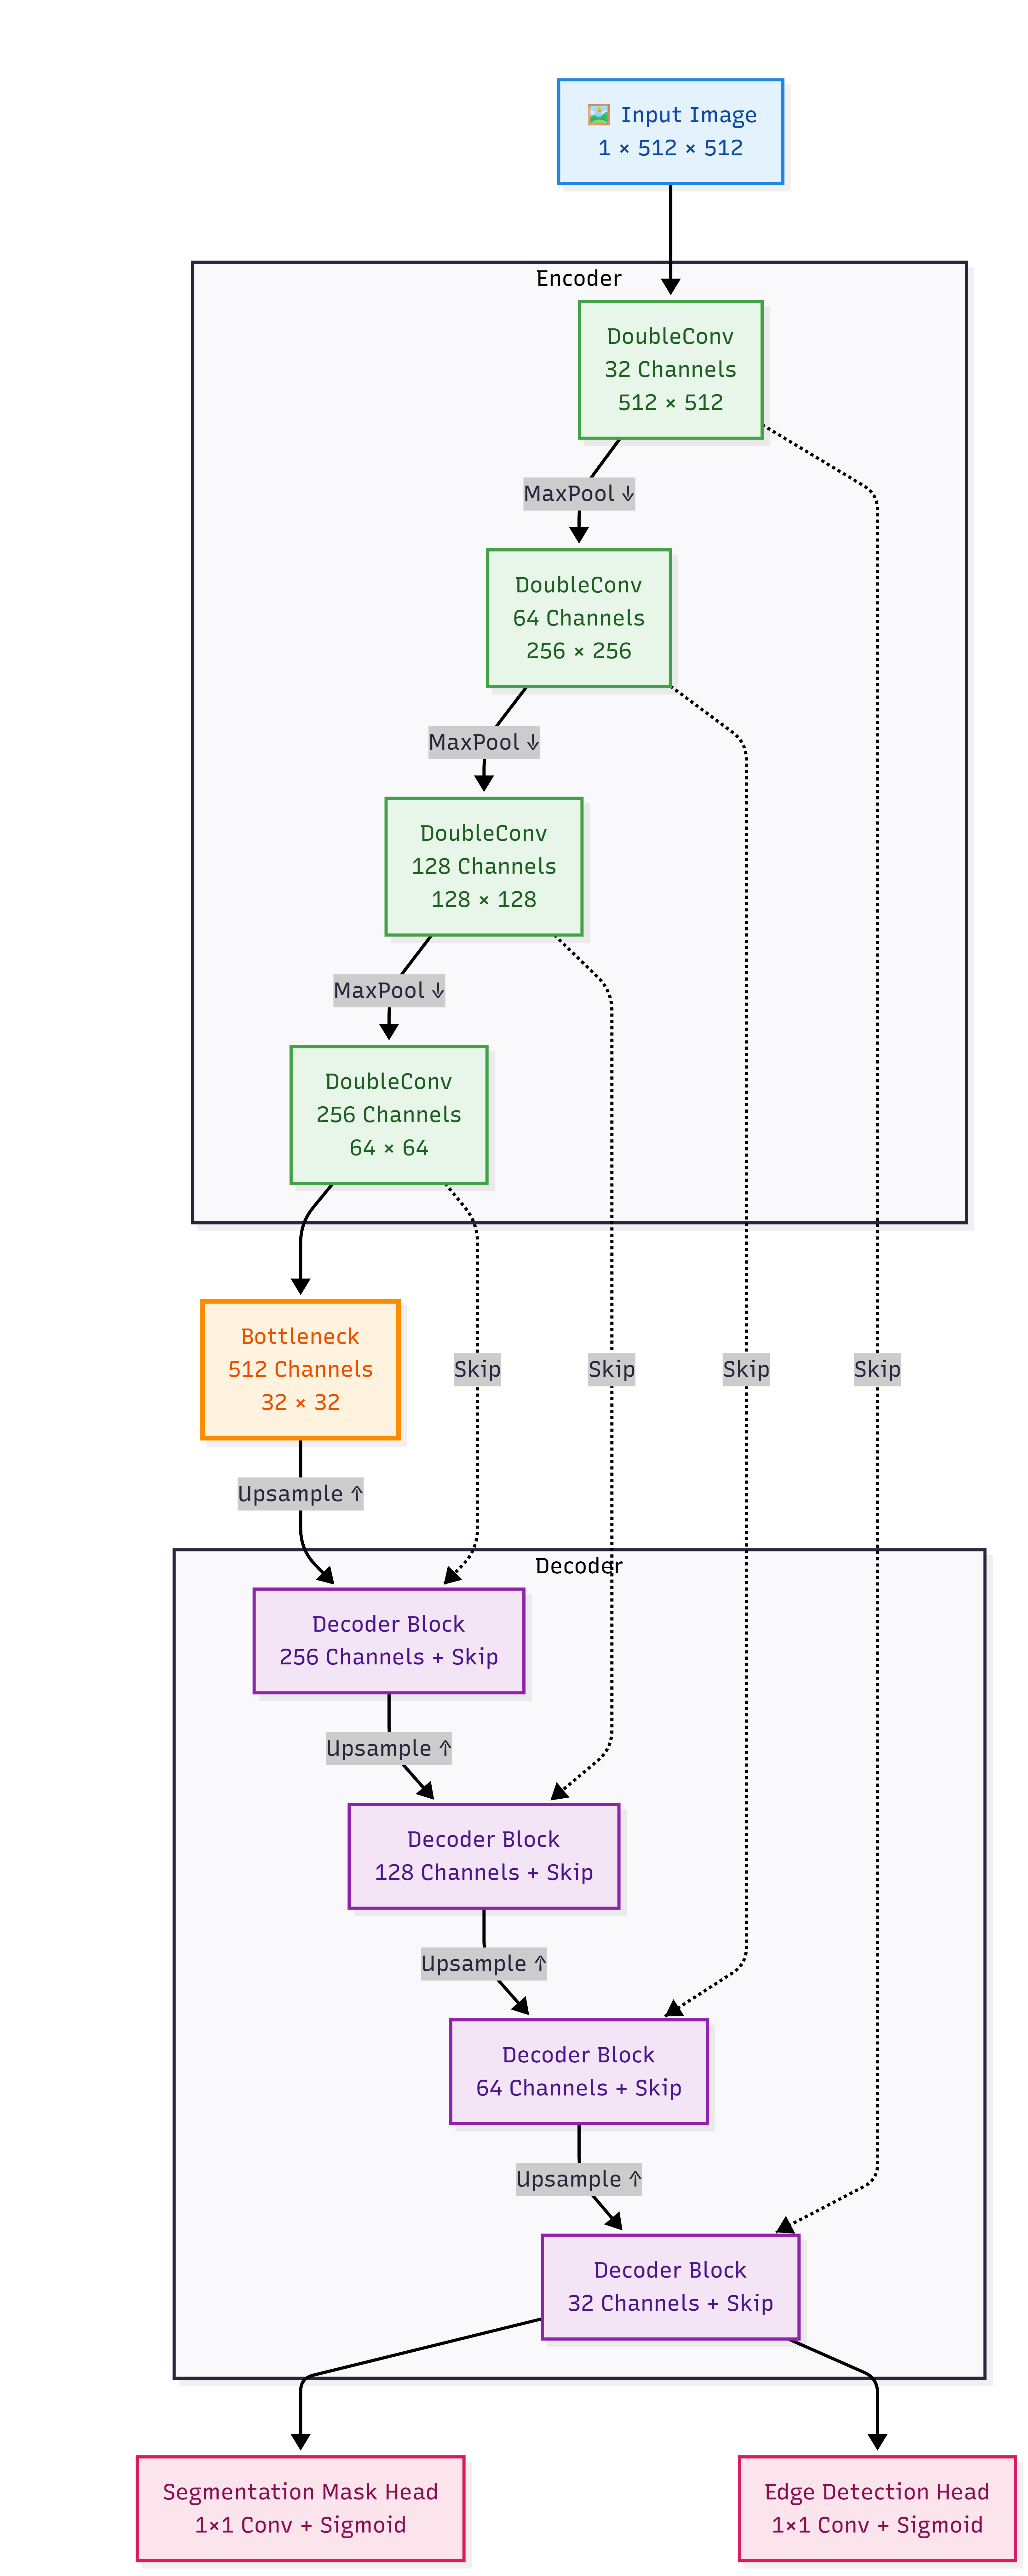
\includegraphics[
        width=\textwidth,
        height=0.92\textheight,
        keepaspectratio
    ]{Chapter3/unetarchitecture.png}
    \caption{Edge-Aware U-Net for lung segmentation with dual mask and edge output heads.}
    \label{fig:unet_arch}
\end{figure}
%------------------------------------------------------------------
\section{Normalization}
%------------------------------------------------------------------

All images are normalized using ImageNet statistics to align with the pretrained EfficientNet-B3 weights:

\[
\mu = [0.485,\ 0.456,\ 0.406], \quad \sigma = [0.229,\ 0.224,\ 0.225]
\]

The normalization is applied as the final step of every image transformation pipeline:

\begin{lstlisting}[style=pythonstyle, caption={Standard ImageNet normalization}]
transforms.Normalize([0.485, 0.456, 0.406],
                     [0.229, 0.224, 0.225])
\end{lstlisting}

Additionally, the patient age values have been clipped to the range $[0, 100]$ and divided by 100 to yield a normalized scalar in $[0,1]$, ensuring consistent numerical scale across metadata features.

For the segmentation model, images are normalized independently with mean $0.5$ and standard deviation $0.5$ since the U-Net is trained from scratch on grayscale inputs and does not use ImageNet pretrained weights.

%------------------------------------------------------------------
\section{Data Augmentation}
%------------------------------------------------------------------

Two distinct augmentation pipelines are used depending on the class frequency of each sample.

\subsection{Standard Augmentation (Common Classes)}

\begin{lstlisting}[style=pythonstyle, caption={Standard augmentation pipeline}]
common_transform = transforms.Compose([
    transforms.Resize((448, 448)),
    transforms.RandomHorizontalFlip(),
    transforms.ToTensor(),
    transforms.Normalize([0.485, 0.456, 0.406],
                         [0.229, 0.224, 0.225])
])
\end{lstlisting}

\subsection{Heavy Augmentation (Rare Classes)}

For rare pathologies such as Hernia, Fibrosis, and Emphysema, a heavier augmentation strategy is applied to synthetically increase sample diversity. This ensures that the model is able to generalize well even over diseases that aren't seen very often.

These are the Heavy transforms applied in order
\begin{enumerate}
    \item Resize
    \item Random Horizontal Flip
    \item Random Rotation (±20°)
    \item Random Resized Crop (Zoom 0.8–1.0)
    \item Random Affine Translation (10%)
    \item Color Jitter (Brightness, Contrast, Saturation)
    \item ToTensor 
    \item Normalize

\end{enumerate}

\subsection{SSL Augmentation (Two-View Contrastive)}

For OPTiML-inspired self-supervised pretraining, a two-view stochastic augmentation pipeline is applied to each image, generating a pair $(X_1, X_2)$. Gaussian noise is added as a final touch.

\subsection{Bounding Box Augmentation}

A critical design constraint for the localization pipeline is that all geometric augmentations (horizontal flip, random rotation, random crop, affine translation) must be \emph{removed} from the training transforms. These operations move pixels without updating the bounding box targets, corrupting the supervision signal. The localization training pipeline therefore uses only photometric transforms:

\begin{enumerate}
    \item Resize to $448 \times 448$
    \item ColorJitter (brightness $\pm 0.2$, contrast $\pm 0.2$, saturation $\pm 0.1$)
    \item ToTensor and ImageNet normalization
\end{enumerate}

\subsection{Segmentation Augmentation}

Joint augmentation is applied identically to the image and its corresponding mask to maintain spatial consistency. Only transforms that preserve the mask-pixel correspondence are used:

\begin{enumerate}
    \item Horizontal Flip (p=0.5)
    \item Rotation (±10°, constant border padding)
    \item Random Brightness/Contrast ($\pm 0.15$)
    \item Resize to $512 \times 512$
    \item Normalize (mean=0.5, std=0.5)
\end{enumerate}

A progressive unfreezing strategy is applied: the EfficientNet backbone is initially frozen so only the classification head is trained. At epoch 6, all backbone parameters are unfrozen and the learning rate is reduced to $10^{-5}$, this is in sync with the SSL+SL pretraining that was done which formed the backbone of bbox localization task.

For the SSL pretraining stage, \textbf{AdamW} is used with a lower weight decay to preserve spatial feature quality:

%------------------------------------------------------------------
\section{Loss Function}
%------------------------------------------------------------------

\subsection{Focal Loss for Supervised Classification}

Given the severe class imbalance in the NIH chest X-ray dataset, a \textbf{Multi-label Focal Loss} is used instead of usual Binary Cross-Entropy. The focal loss down-weights easy, well-classified examples and focuses learning on hard and misclassified samples:

\begin{equation}
\mathcal{L}_{\text{Focal}} = -\alpha \sum_{i} (1 - p_t)^{\gamma} \cdot \text{BCE}(\hat{y}_i, y_i)
\end{equation}

where $p_t = \sigma(\hat{y}_i)$ if $y_i = 1$, else $p_t = 1 - \sigma(\hat{y}_i)$, and $\alpha = 0.25$, $\gamma = 2.0$.

\subsection{OPTiML-Inspired SSL Loss}

The self-supervised pretraining stage uses a composite loss combining three components:

\subsubsection{Optimal Transport (OT) Structural Alignment~\cite{otcxr}}

Given two sets of dense patch embeddings $\mathbf{z}_1, \mathbf{z}_2 \in \mathbb{R}^{B \times HW \times D}$, a Sinkhorn-regularized optimal transport plan $\mathbf{T}$ is computed and the transport cost minimized.
\newline
Optimal Transport can be defined as the how can we align one geometry with the other with minimum cost possible so in our case we are using two augmented view so our problem is how can we align these two images probabilistically, now we can see it is somewhat similar to KL divergence but the key features that OT provides and is good for our use case is that it works at patch level and can align spatial structures whereas KL requires supports to overlap.
\begin{equation}
\mathcal{L}_{\text{OT}} = \sum_{i,j} T_{ij} \cdot C_{ij}, \quad C_{ij} = 1 - \cos\left(\mathbf{z}_{1,i},\ \mathbf{z}_{2,j}\right)
\end{equation}


\subsubsection{Variance Regularization~\cite{otcxr}}

Encourages representation diversity by penalizing collapsed feature dimensions:

\begin{equation}
\mathcal{L}_{\text{var}} = \mathbb{E}_d \left[\max\!\left(0,\ 1 - \sqrt{\mathrm{Var}_n(z_{n,d}) + \epsilon}\right)\right]
\end{equation}


\subsubsection{Covariance Regularization~\cite{otcxr}}

Decorrelates feature dimensions to reduce redundancy, following the Barlow Twins principle:

\begin{equation}
\mathcal{L}_{\text{cov}} = \frac{1}{D} \sum_{i \neq j} \left[\frac{(\mathbf{z}^\top \mathbf{z})_{ij}}{N-1}\right]^2
\end{equation}



\subsubsection{Total SSL Loss}

The complete SSL objective is:

\begin{equation}
\mathcal{L}_{\text{SSL}} = \mathcal{L}_{\text{OT}} + \lambda_{\text{var}} \cdot \mathcal{L}_{\text{var}} + \lambda_{\text{cov}} \cdot \mathcal{L}_{\text{cov}}
\end{equation}

with $\lambda_{\text{var}} = 0.1$ and $\lambda_{\text{cov}} = 0.01$.

\subsection{CIoU Loss for Bounding Box Regression}

Standard mean-squared error treats all coordinate errors equally regardless of box size. A \textbf{Combined Loss} of Complete IoU (CIoU) and Smooth-L1 is used instead:

\begin{equation}
\mathcal{L}_{\text{bbox}} = \mathcal{L}_{\text{CIoU}} + 0.5 \cdot \mathcal{L}_{\text{SmoothL1}}
\end{equation}

CIoU extends the standard IoU loss with a centre-distance penalty and an aspect-ratio consistency term:

\begin{equation}
\mathcal{L}_{\text{CIoU}} = 1 - \text{IoU} + \frac{d^2}{c^2} + \alpha v
\end{equation}

where $d^2$ is the squared Euclidean distance between predicted and target centres, $c^2$ is the squared diagonal of the smallest enclosing box, $v = \frac{4}{\pi^2}(\arctan\frac{w^{gt}}{h^{gt}} - \arctan\frac{\hat{w}}{\hat{h}})^2$ penalizes aspect-ratio mismatch, and $\alpha = v / (1 - \text{IoU} + v)$ is an adaptive weighting factor. The Smooth-L1 component provides stable gradient signal when predictions are far from targets.

\subsection{Segmentation Loss}

The total segmentation loss combines three terms:

\begin{equation}
\mathcal{L}_{\text{seg}} = \mathcal{L}_{\text{Dice}} + \mathcal{L}_{\text{BCE}}^{\text{boundary}} + \lambda_e \cdot \mathcal{L}_{\text{edge}}
\end{equation}

\paragraph{Dice Loss} addresses foreground-background imbalance by optimizing overlap directly:
\begin{equation}
\mathcal{L}_{\text{Dice}} = 1 - \frac{2\sum_i \hat{M}_i M_i + \epsilon}{\sum_i \hat{M}_i + \sum_i M_i + \epsilon}
\end{equation}

\paragraph{Boundary-Weighted BCE} amplifies the gradient signal at lung boundary pixels by upweighting them in the pixel-wise cross-entropy, encouraging sharper contours:
\begin{equation}
\mathcal{L}_{\text{BCE}}^{\text{boundary}} = \frac{1}{N}\sum_i (1 + \alpha \cdot E_i^{gt}) \cdot \text{BCE}(\hat{M}_i, M_i)
\end{equation}
where $E^{gt}$ is the ground-truth binary edge map and $\alpha = 5.0$ is the boundary amplification factor.

\paragraph{Edge Head Loss} directly supervises the auxiliary edge prediction branch:
\begin{equation}
\mathcal{L}_{\text{edge}} = \text{BCE}(\hat{E},\ E^{gt}), \quad \lambda_e = 0.3
\end{equation}

\subsection{Early Stopping}

To prevent overfitting, early stopping monitors validation AUC with a patience of 5 epochs and a minimum improvement delta of $10^{-4}$, this was removed to train SSL.

%------------------------------------------------------------------
\section{Post-Processing and Zone-Based Report Generation}
%------------------------------------------------------------------

\subsection{Segmentation Post-Processing}

Raw sigmoid probability maps from the U-Net are refined through a three-step pipeline before being used for zone extraction:

\begin{enumerate}
    \item \textbf{Threshold at 0.5} to produce a binary mask.
    \item \textbf{Morphological closing} (elliptical kernel, $k=7$, two iterations) to fill intra-lung holes introduced by vessels or airways and other silhouette overlap.
    \item \textbf{Connected-component filtering}: components smaller than 1,000 pixels are discarded; only the two largest remaining blobs (corresponding to the left and right lung) are retained.
\end{enumerate}

\subsection{Left/Right Lung Extraction and Zone Division}

The two boxes that surround the lungs are then assigned to left and right lungs by centroid $x$-coordinate following general convention: the patient's \emph{right} lung appears on the image \emph{left} (smaller centroid $x$), and the patient's \emph{left} lung appears on the image \emph{right} (larger centroid $x$).

Each lung bounding box is then divided into three equal horizontal thirds, yielding six zones that can be used for report generation:

\begin{table}[ht]
\centering
\caption{Anatomical zone nomenclature derived from segmented lung bounding boxes.}
\label{tab:zones}
\renewcommand{\arraystretch}{1.3}
\begin{tabular}{cll}
\toprule
\textbf{Zone Code} & \textbf{Full Name} & \textbf{Vertical Extent} \\
\midrule
RUZ & Right Upper Zone  & $y_1$ to $y_1 + \frac{H}{3}$ \\
RMZ & Right Middle Zone & $y_1 + \frac{H}{3}$ to $y_1 + \frac{2H}{3}$ \\
RLZ & Right Lower Zone  & $y_1 + \frac{2H}{3}$ to $y_2$ \\
LUZ & Left Upper Zone   & $y_1$ to $y_1 + \frac{H}{3}$ \\
LMZ & Left Middle Zone  & $y_1 + \frac{H}{3}$ to $y_1 + \frac{2H}{3}$ \\
LLZ & Left Lower Zone   & $y_1 + \frac{2H}{3}$ to $y_2$ \\
\bottomrule
\end{tabular}
\end{table}

Each detected disease is assigned to the zone with maximum bounding box intersection area, computed as the overlap between the disease bounding box (from the regressor) and each of the six zones, with the argmax zone selected.

\subsection{Structured Radiology Report Generation}

The final pipeline stage synthesizes outputs from all three models into a structured, template-driven report organized into five sections mirroring clinical reporting conventions:

\begin{enumerate}
    \item \textbf{Patient Information:} Study date, image filename, age, sex, and view position.
    \item \textbf{Findings Summary:} A concise list of all detected diseases with their classifier confidence scores.
    \item \textbf{Lung Field Assessment:} Reports whether each lung field was successfully segmented and provides bounding box coordinates for reference.
    \item \textbf{Zonal Analysis:} For each of the six zones (RUZ, RMZ, RLZ, LUZ, LMZ, LLZ), reports either the associated disease(s) with confidence or ``Appears normal.''
    \item \textbf{Impression:} A concise summary automatically detecting bilateral conditions (present in both left and right zones) and generating clinically phrased sentences.
\end{enumerate}

Rather than applying a global threshold to all disease probabilities, \textbf{per-class thresholds} are optimized on the validation set by maximizing macro-averaged F1 independently for each disease label. This is especially important for rare pathologies where the default 0.5 threshold produces trivially low recall.

\begin{lstlisting}[style=pythonstyle, caption={Sample generated radiology report (truncated)}]
======================================================================
                   CHEST X-RAY ANALYSIS REPORT
======================================================================
PATIENT INFORMATION
  Age: 69 years  |  Sex: Female  |  View: PA

FINDINGS SUMMARY
  Detected conditions (2):
    * Effusion      (confidence: 78.3%)
    * Atelectasis   (confidence: 65.1%)

ZONAL ANALYSIS
  Right Lower Zone  : Possible sign of Effusion (78.3%)
  Left Middle Zone  : Possible sign of Atelectasis (65.1%)
  [all other zones] : Appears normal

IMPRESSION
  * Effusion in the Right Lower Zone
  * Atelectasis in the Left Middle Zone
----------------------------------------------------------------------
  WARNING: AI-generated. Requires radiologist verification.
======================================================================
\end{lstlisting}

\begin{figure}[ht]
    \centering
    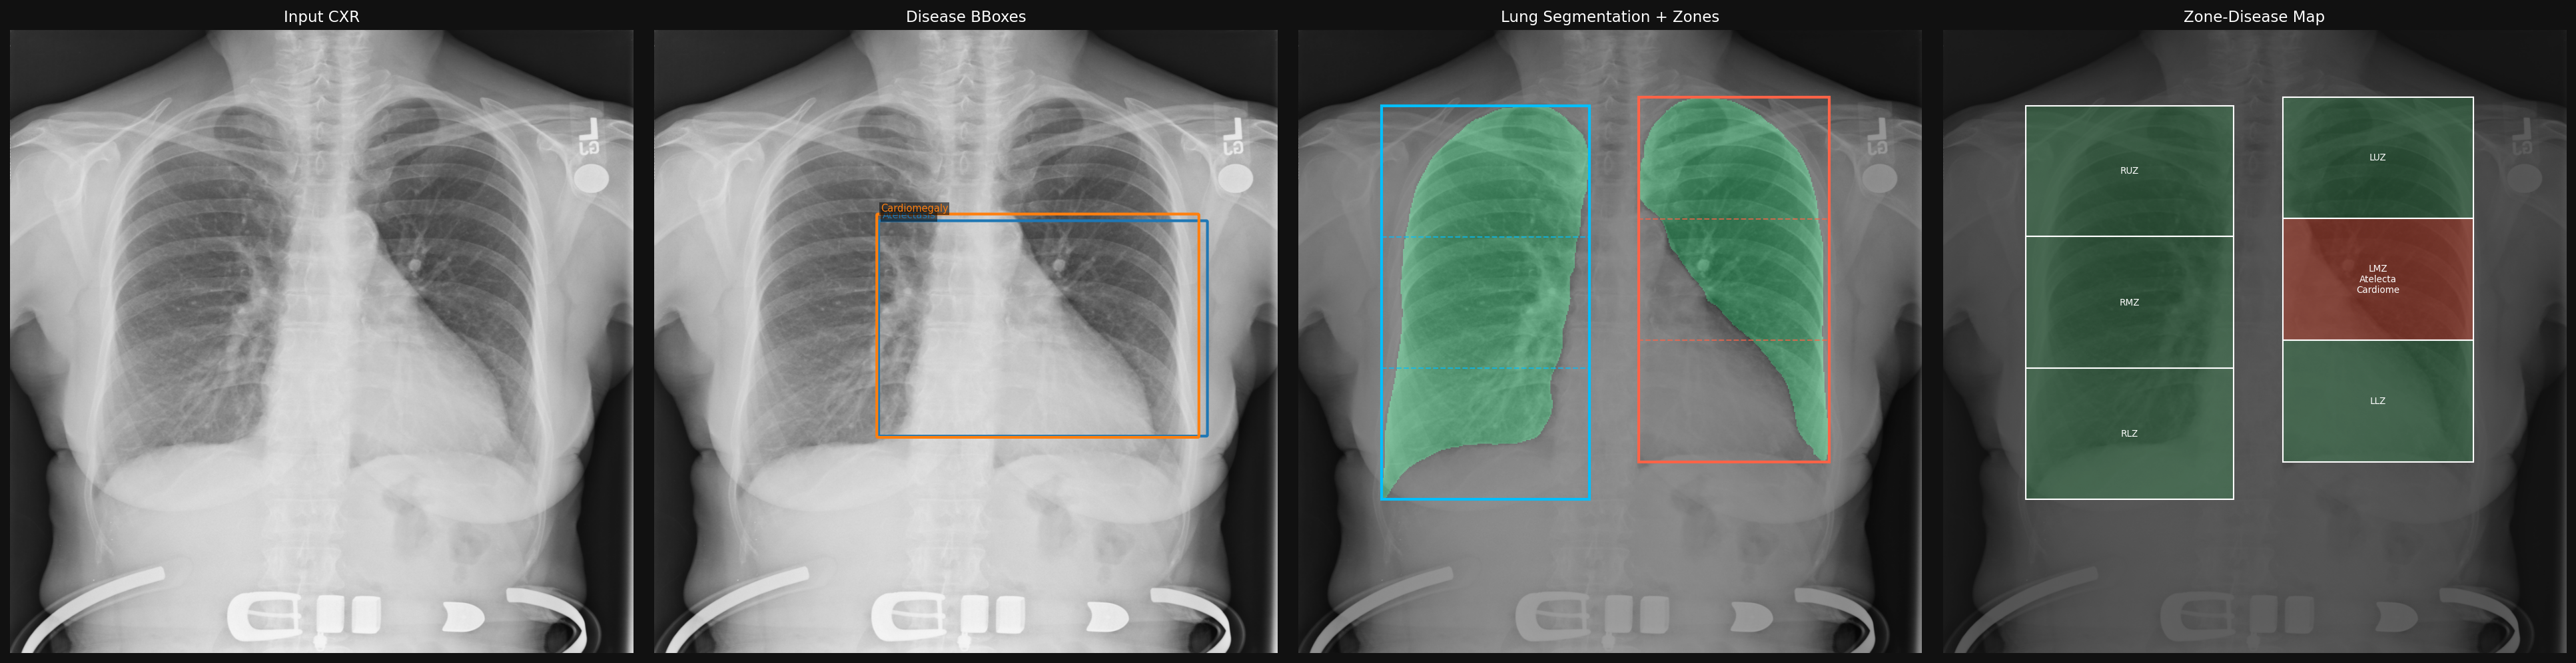
\includegraphics[
        width=\textwidth,
        height=0.99\textheight,
        keepaspectratio
    ]{Chapter3/pipeline_result.png}
    \caption{Four-panel visualisation of the complete inference pipeline on a sample NIH chest radiograph.}
    \label{fig:pipeline_viz}
\end{figure}

\begin{figure}[ht]
    \centering
    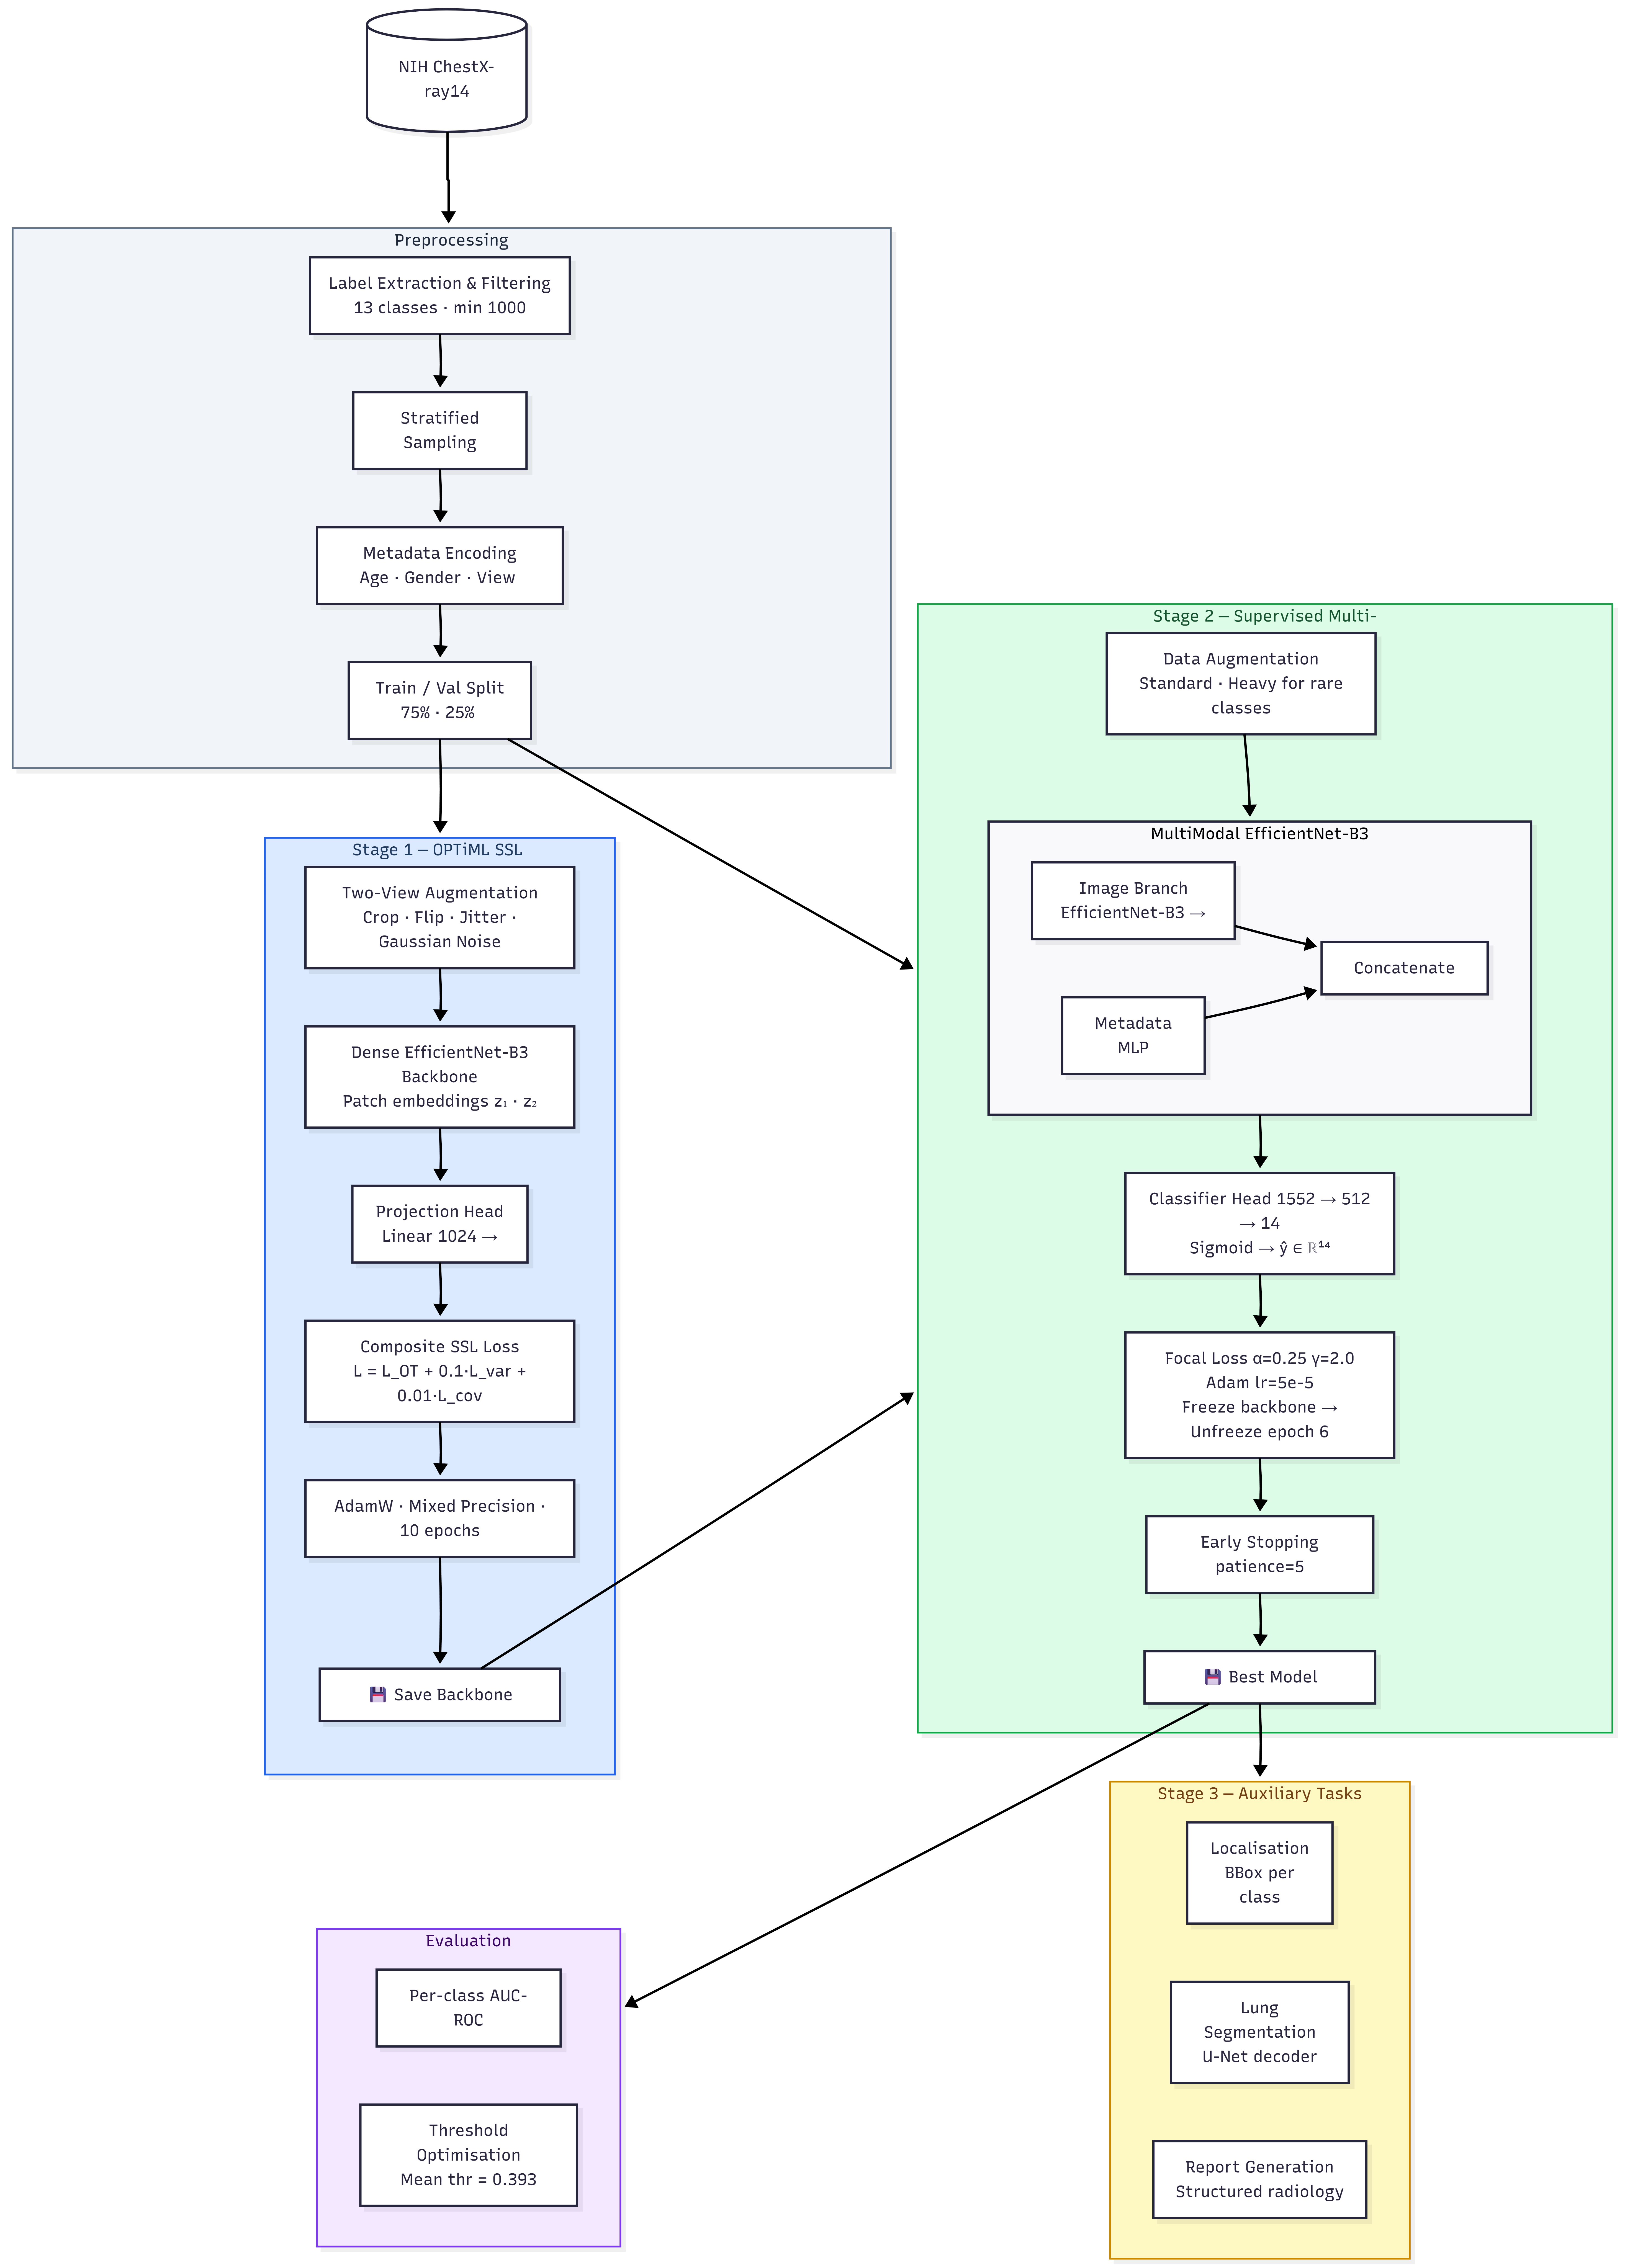
\includegraphics[width=\textwidth]{Chapter3/architecture_flow.png}
    \caption{Overall system architecture.}
    \label{fig:architecture}
\end{figure}